%%%%%%%%%%%%%%%%%%%%%%%%%%%%%%%%%%%%%%%%%%%%%%%%%%%%%%%%%%%%%%%%%
%%%  Capstone Project Template that tries to save a few trees %%%
%%%  Edwin Blake 22 Aug 2013                                                   %%%
%%%		1 Aug 2014 (revised)                                      %%% 
%%%  see also                                                                             %%%
%%% http://ravirao.wordpress.com/2005/11/19/latex-tips-to-meet-publication-page-limits/  
%%%%%%%%%%%%%%%%%%%%%%%%%%%%%%%%%%%%%%%%%%%%%%%%%%%%%%%%%%%%%%%%%

\documentclass[11pt,a4paper]{article}
\usepackage{times}
\usepackage{fancyhdr}           % Allows better control over headers and footers
%\usepackage{layout}            % use with \layout to see the page layout for
%debugging purposes.
\usepackage[margin=2.5cm]{geometry}  %   set the margins using the
                                %   geometry package (which is much
                                %   the easiest way of doing this).
\usepackage[pdftex]{graphicx}   %   Pictures (means you have to
                                %   produce pdf output via pdflatex)
\usepackage[small,compact]{titlesec}   % Try to reduce the white space
                                % latex loves so much
\titlelabel{\thetitle. \quad}   % Reduce space around section heads
                                % and add a full stop after the number
\pagestyle{fancy}               % Invoke fancy headers

\renewcommand{\abstractname}{\vskip -5mm}  %  Change name of Abstract
                                %  to nothing and loose some of the
                                %  excessive white space
\usepackage{float}


\begin{document}

\title{Cheaters Plagiarism Detection Report} \date{}
\author{Merishka Lalla\\joe@bloggs.com
\and Yaseen Hamdulay\\jane.doe@uct.ac.za
\and Jarred de Beer\\john.doe@uct.ac.za}

%%%  Set the headers via fancyhdr package
\lhead{Capstone Project Report}  % Short title for running head
\chead{}
\rhead{1st August, 2014}   %  Fixed running head of the date
\lfoot{}
\cfoot{\thepage}    %  add page number as centre footer.
\rfoot{}
\renewcommand{\headrulewidth}{0.0pt}   % Don't want horizontal line
                                % under header.

\maketitle
\thispagestyle{plain}  % First page is plain style headings and
                       % footers (ie just the page number as footer).

\section*{Abstract}
The purpose of this project is to identify cheating among Computer Science
students when submitting their assignments. It is estimated that
30\% of students will cheat in an assignment, often sharing the code in groups amongst themselves.
 Our goal is to detect such occurrences and display the results for lecturer administration. 
We began by building a prototype, basing the algorithm on the proprietary JMoss system, 
but using only Python. We found our implementation worked well but failed in that it detected single lines 
of common and insignificant code, also, the initial UI could not display the high number of results
being listed. After refactoring our solution was to perform String matching, generating 
signatures on the text and filtering them for multiple lines of
recurring code, further comparing it with as an abstract syntax tree for subtree pattern matching. 
To test the algorithm was run against 18658 python assignments, yielding the same 30\% mean
of students cheating and deviating on the confidence interval with each occurrence by just 0.5\%
as given by the JMoss system. In conclusion our solution performs alongside JMoss, yet differs in its UI by
grouping cheaters to recurring code blocks, a more convenient view to administer cheating.



The purpose of this project is to identify cheating among Computer Science
students when submitting their assignments. It is estimated that 30\% of
students will cheat in an assignment, often sharing the code in groups amongst
themselves. Our goal is to detect such occurrences and display the results for
lecturer administration. With the use of various data structures and algorithms,
the final implementation supports code detection from Java and Python
submissions. This project attempts to be similar to JMoss with the main
difference being that the project has a more interactive user interface with
data presented in alternate forms. The main algorithm was based on the
proprietary JMoss system which can handle a large number of code submissions and
evaluate them, finding the percentage of copied lines out of an assignment.
Development was done using horizontal and evolutionary prototyping. Horizontal
due to the initial broad functionality that was implemented for the prototype
and evolutionary because of the constant changes that were adopted. Testing the
algorithm was done against 18658 python assignments extracted out of the
provided JMoss results. We're happy with the performance of the system, and
believe it performs alongside JMoss, but differs with it's UI and presentation
of data.

\section{Introduction}
\label{s:introduction}

Reuse of code by students in an academic institution is a growing problem due to
the fact that manual detection can be time consuming and finding an algorithm
to detect plagiarism in large repositories is hard to scale\cite{Burrow}.The aim
of this project has been to attempt to find similarities in code which can be
considered cheating and thusly plagiarism in some form. The detection system
plugs in to the student submission process on Vula and will extract the source
files to generate signatures on the source code and match it with existing
signatures. The methodology relates to that of the winnowing algorithm which
generates a digital fingerprint\cite{frohlich}. A front end web UI was built to list the offending students and provide administration functionality for the convening lecturer to take action when needed. The web UI could be accessed from within an iframe in the Vula dashboard or its external URL, by convening lecturers. Lecturers will use this facility to verify code diffs against students' code, mark them as having cheated and be provided with a list of the marked students that they can use to reference when assigning a student zero for an assignment.

The programming languages used for assignments differ from year to year, and in some cases even within the same year. It was therefore necessary to detect the appropriate programming language used with each submission. The Computer Science department makes extensive use of Python and Java for assignments and so these are provided as plugins by default. The system has a plugin sub-system which can be used to write parsers for additional languages, extending the scope of languages used to detect cheating from within the department and allowing flexibility in terms of language support for the future.

The software engineering methods used for the project were traditional analysis followed by design and implementation. An evolutionary prototype was constructed and presented to the stakeholders for review. Given their feedback, we decided to make extensive use of Extreme programming to iterate over the product and get it into its final state. One of the benefits to this technique, in a group of three, was provided by pair programming which allowed any combination of pairs from the group of three to always have at least one member with an up to date, working knowledge of the code and state of the project. This was advantageous especially when refactoring large bodies of code, occurring from technical issues that had became apparent. We were able to discuss such issues immediately, design and implement alternate solutions, and modify existing methods or classes. The source code was checked out from a git repository and the team members could then conveniently update their source code copies after a peer programming session and work on the files individually, safely pushing detailed commits with changes for other team members to remain up to date.

The core of the system, the algorithm detection, is based largely on the proprietary
JMoss system and was referenced while building the Winnowing algorithm as part of the
signature generation and matching. We were able to use the output from a provided database of over 18000 python assignment files from the 1st year Computer Science course and compare our implementation to the results given by JMoss on the same files. This was used also for tweaking parameters to the system and gaining accuracy

\section{Requirements Captured}

\subsection{Use Cases}

Actors: Students and lecturers

The typical scenario is a student submits an assignment through Vula. Once submitted, the assignment is checked against all other submitted assignments for cheating and the result is stored in a database. The lecturer can access the results at any given time to verify cheating.

In the event that a student submits a .zip folder with a syntax error or an unsupported language, the submission will be ignored. It is assumed that syntax errors in submissions would result in 0 from the automatic marker and also from tutors trying to run them.

\begin{figure}[H]
  \center{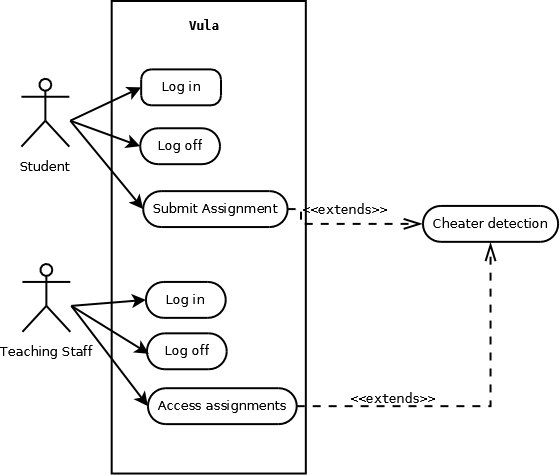
\includegraphics[width=400px]{use_case.png}}
  \caption{A use case diagram illustrating system interaction}
  \label{fig:usecase}
\end{figure}

\subsection{Functional Requirements}

\paragraph{Data integrity}
\begin{itemize}
    \item Data provided to the database must be correct, complete and coherent
    \item Data must be easily accessed whenever necessary
    \item Automated report generation with correct data
\end{itemize}

\paragraph{Information retrieval}
\begin{itemize}
    \item Retrieve matching pairs
    \item Retrieve list of marked cheated students
\end{itemize}

\paragraph{Authentication}
\begin{itemize}
    \item Must be accessible to UCT computer science students only
\end{itemize}

\paragraph{Database management}
\begin{itemize}
    \item General upkeep of database
    \item Store relevant data in a normalised format
\end{itemize}

\paragraph{Security}
\begin{itemize}
    \item Cheater checker data must be unavailable to students after they check their submissions.
    \item If security is breached, the software becomes redundant
\end{itemize}

\subsection{Non-functional Requirements}

\paragraph{Performance}
\begin{itemize}
    \item Cheater checker should be able to compute and check submissions within O(logN) 
\end{itemize}

\paragraph{Availability}
\begin{itemize}
    \item Must be available by lecturers even if Vula is down
\end{itemize}

\paragraph{Usability}
\begin{itemize}
    \item All users must be able to use the software easily because of an intuitive design
\end{itemize}

\paragraph{Capacity}
\begin{itemize}
    \item Must be able to handle the instance of all student submitting at once
\end{itemize}

\subsection{Usability Requirements}

\paragraph{Understandability}
\begin{itemize}
    \item Intuitive UI
    \item Easily understood results
    \item Easily identify Pairs of students with high likelihood of cheating from a list
    \item Easily identify Groups of students with high likelihood of cheating from a list
\end{itemize}

\paragraph{Learnability}
\begin{itemize}
    \item Complete documentation will be provided
    \item Explanation on how the system works for the designed context
    \item System relies on users recall rather than recognition
\end{itemize}

\paragraph{Operability}
\begin{itemize}
    \item Consistent UI elements
    \item Responsive UI interaction elements
    \item Reversible actions and constant feedback given 
    \item Responsive User interface design to accommodate varying screen resolutions
    \item Record students as having cheated individually from a Pair of students
    \item View list of students recorded for cheating to take action on them, instead of manually maintaining a spreadsheet.
\end{itemize}

\subsection{Artefacts produced}

\begin{figure}[H]
  \center{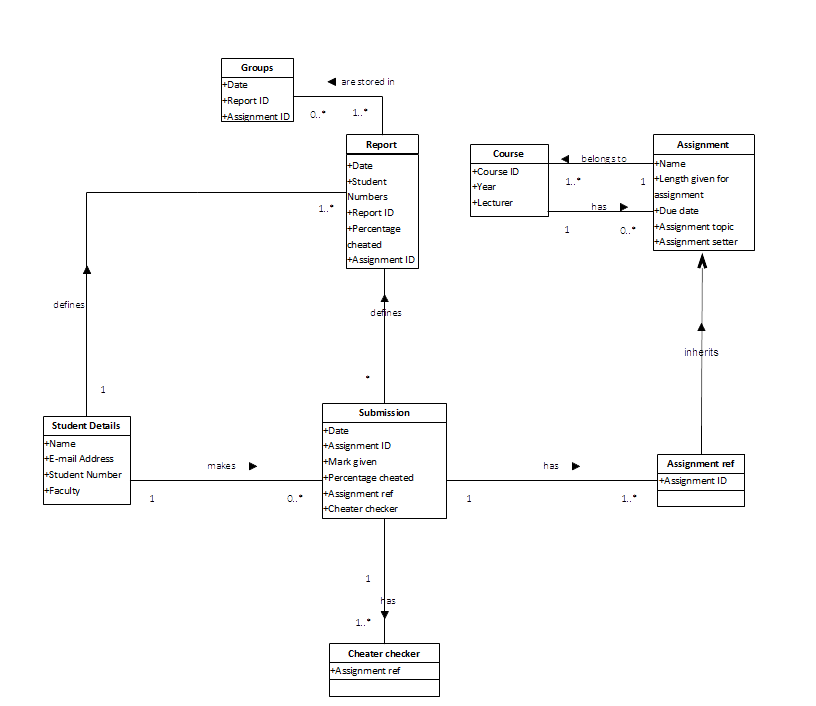
\includegraphics[width=\textwidth]{analysis_class.png}}
  \caption{Analysis Class Diagram}
  \label{fig:analysisclass}
\end{figure}

A risk management assessment, relevant diagrams (such as class diagrams and
architectural diagrams) and a gantt chart were produced in order to aid the
development process with respect to time management and general direction. 

\section{Design Overview}
\label{s:design-overview}

The UI may be embedded within an existing system such as Vula and it does not
have to be used from an external URL endpoint. The system plugs into Vula to
receive submissions. It then generates and stores signatures on the submission
which get processed by a separate service that identifies matches and stores
them. A lecturer reviews the results from the matches in the presentation layer and makes a decision as to whether the student should be marked for cheating or not. Submissions are categorised by their respective assignment, and are matched against submissions within that assignment over multiple years.

\paragraph{Algorithms used were}
\begin{itemize}
\item The Winnower algorithm (coarse matching)
\item Grouper algorithm
\item Suffix tree algorithm (exact matching)
\end{itemize}

The winnowing algorithm\cite{frohlich} was used to give us coarse but fast
matching between submissions. We used it to generate a signature for each
submission and match that signature with other submission signatures. This tells
us which submission most closely matches another. Due to the coarse nature of the winnowing algorithm we are unable to pull out line information from it. For this we used a Generalised Suffix Tree for more exact substring matching. Generating a suffix tree is a lot slower than the winnower algorithm so it can only be used for finding matches when we already know which pairs of submissions are most similar. We used the generalised suffix tree to find long common substrings and match those between submissions.

We implemented Ukkonen's algorithm to generate the suffix tree in linear time.

Prior to doing any submission matching we strip out all variable names, class
names, method names etc that students may replace to attempt to obfuscate pieces
of plagiarised code.

\paragraph{Algorithms used were}
\begin{itemize}
    \item The Winnower algorithm
    \item Grouper algorithm
    \item Suffix tree algorithm
\end{itemize}

\begin{figure}[H]
  \center{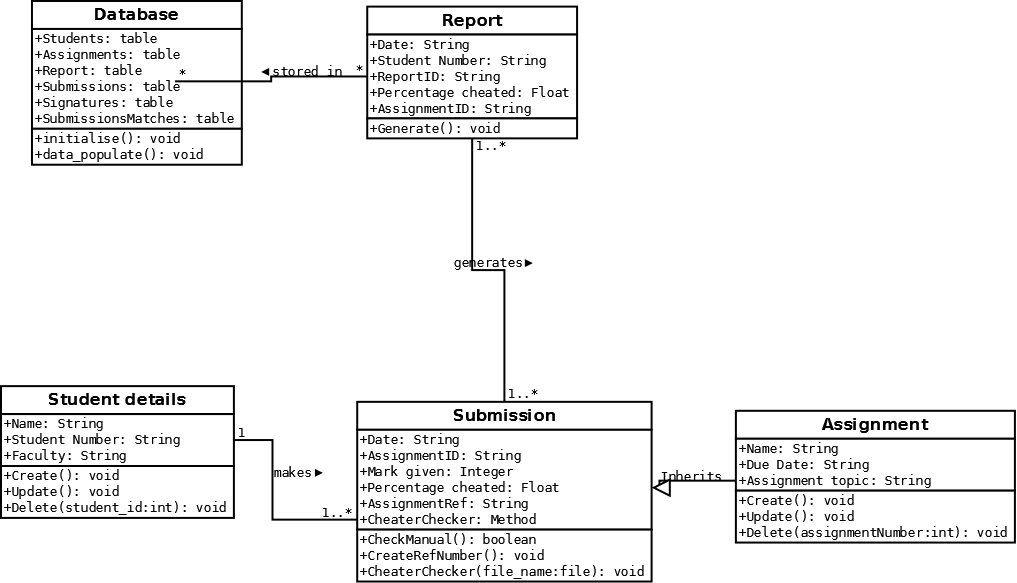
\includegraphics[width=\textwidth]{design_class.png}}
  \caption{Design class diagram}
  \label{fig:designclass}
\end{figure}

\begin{figure}[H]
  \center{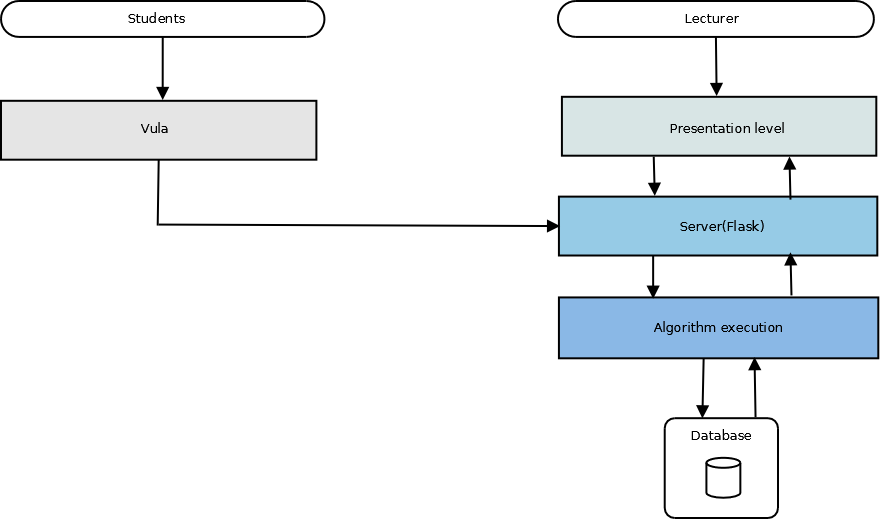
\includegraphics[width=400px]{layered_architecture.png}}
  \caption{Layered architectural diagram}
  \label{fig:layeredarchitecture}
\end{figure}



\section{Implementation}

\subsection{Data structures used}

\begin{figure}[H]
  \center{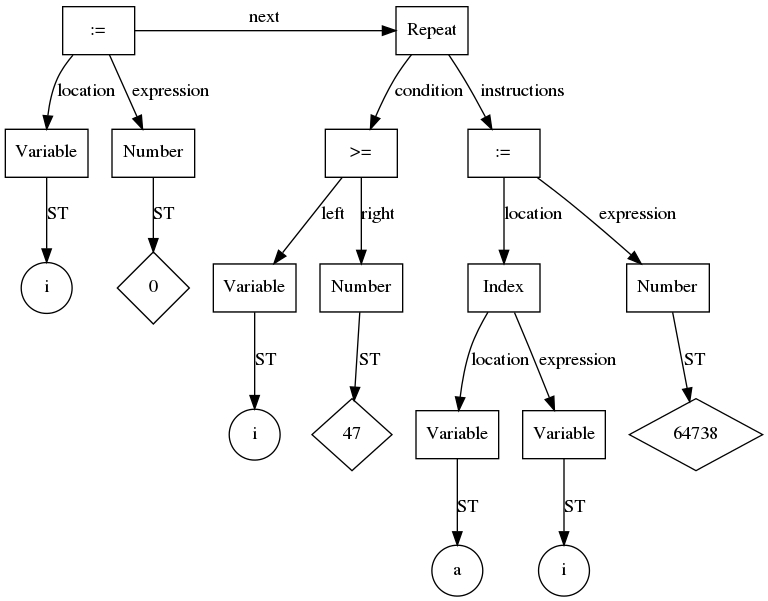
\includegraphics[width=250px]{abstract_syntax_tree.png}}
  \caption{Abstract Syntax Tree\cite{schleimer}}
  \label{fig:abstractsyntaxtree}
\end{figure}

\begin{figure}[H]
  \center{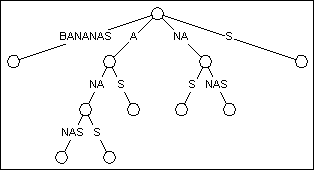
\includegraphics[width=250px]{suffix_tree.png}}
  \caption{Suffix Tree\cite{unknown2}}
  \label{fig:suffixtree}
\end{figure}

The suffix tree is a tree structure which looks at the last part of a
given output. From the example, it gives all possible end combinations. This was
used to find the longest common substring in the code.

\begin{figure}[H]
  \center{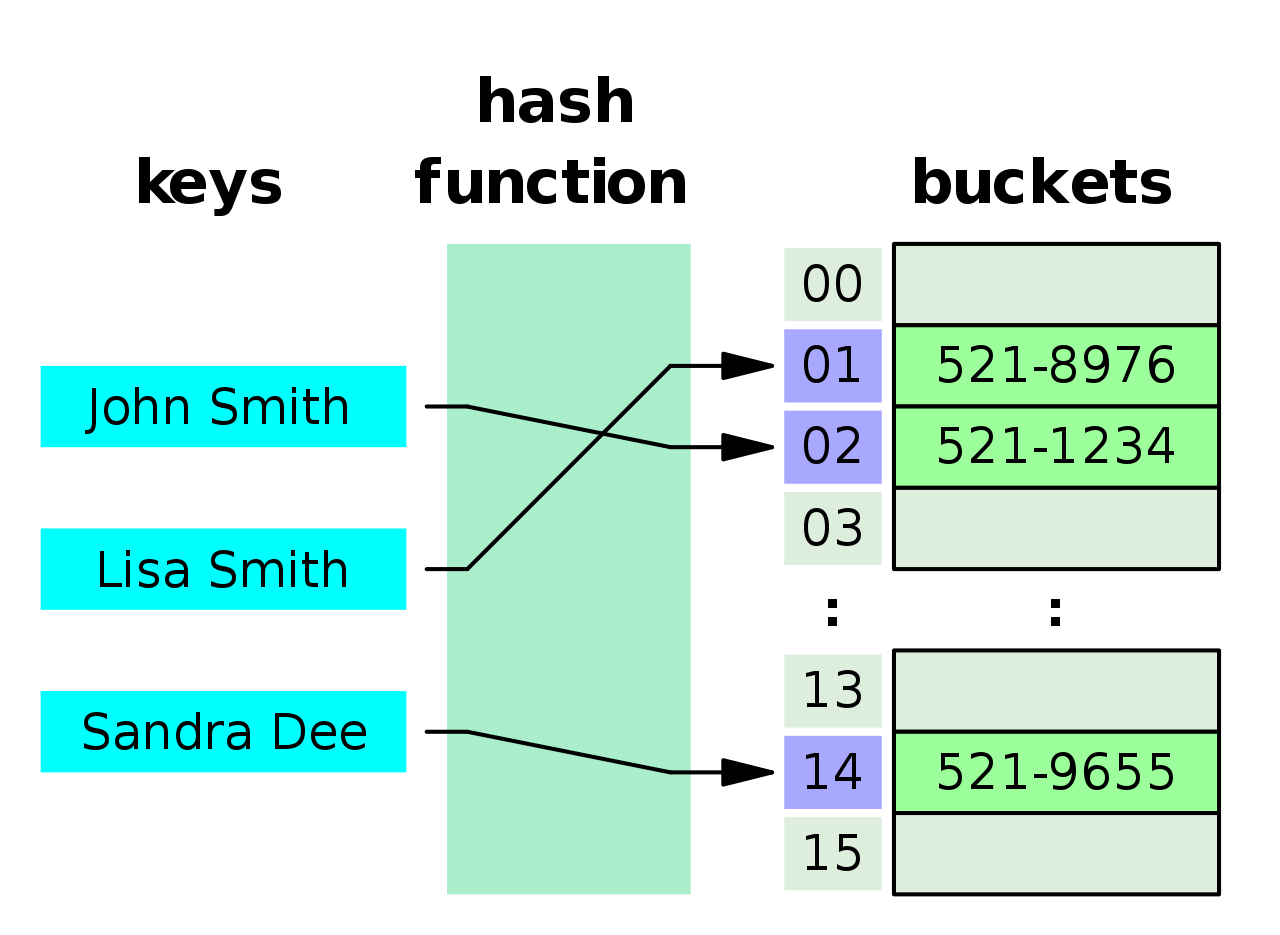
\includegraphics[width=250px]{hash_map.png}}
  \caption{Hash Map\cite{unknown1}}
  \label{fig:hashmap}
\end{figure}

A hash map is used to map keys to values in near constant time. We used hashing to map between identifiers from one suspected instance of cheating to another for a greater measure of accuracy.


\section{User Interface features and implementation}

\begin{figure}[H]
  \center{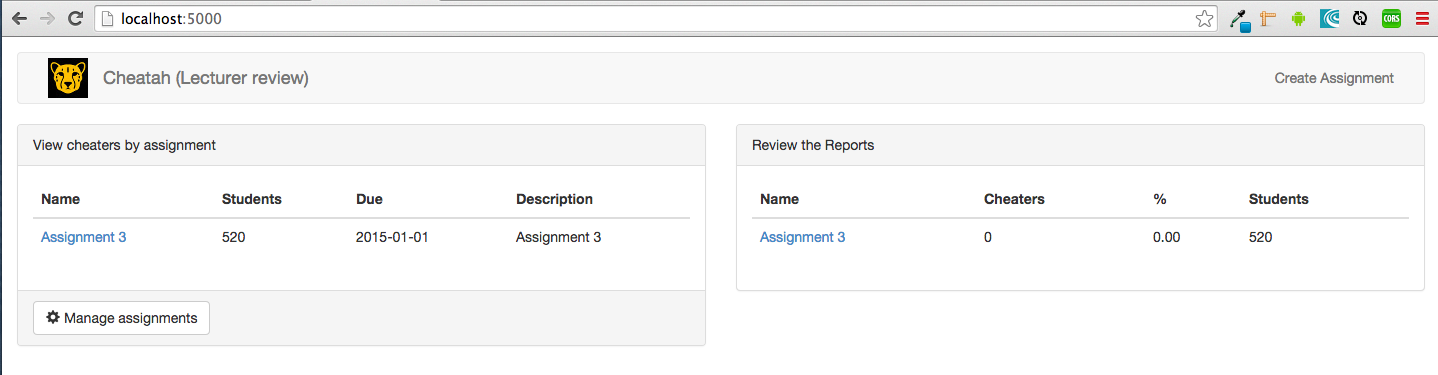
\includegraphics[width=\textwidth]{ui_screenshot.png}}
  \caption{A screenshot of the UI on the home screen}
  \label{fig:uiscreenshot}
\end{figure}

The above image is an example of a screenshot from the home page. The UI was created using HTML and CSS for templating and Javascript for interaction. External libraries such as Bootstrap for CSS, D3.js for graphs, Prism.js for code highlighting, and jQuery were used. The implementation was done using the web framework called Flask.

\subsection{Overall design}

The user interface forms the front-end of the system which is served by the Flask server level and intended to be displayed in a modern browser. The interface was designed to be responsive in both its layout and functionality. It will adapt for optimal view on any reasonable screen resolution, and will also respond quickly to user interaction.  In order to achieve this some considerations needed to be taken into account, with their associated consequences. The biggest issue in supporting user interaction is cross browser compatibility. As this is not a functional requirement for the system, but a direct influence on the user’s ability to interact with it, it remains a critical concern. The following two paragraphs detail the solutions to this. 

The Bootstrap 3 CSS framework was used as a base level of CSS to enforce resets and layout rules that would make the UI responsive and compatible across browsers, backing up to Internet Explorer 8 and 9. On top of this, a style.css file was written to override Bootstrap’s CSS rules where necessary to accomplish the overall design. It was not necessary to make use of all of Bootstrap’s javascript libraries, so this is not included, but we make use of two of its smaller javascript files: alert.js so users can close alert dialogs; and dropdown.js for the dropdown menu in the navigation bar.

The considerations on cross browser javascript support in achieving responsive
user interactions are less forgiving. Javascript runs single threaded in the
browser and as a requirement needs to be non-blocking on the interface. In order
to achieve a responsive and non-blocking interface the UI needs to make any
combination of HTTP requests to the Flask server layer in an asynchronous
manner. Such asynchronous requests are generally written with function calls
that get given, as parameters, callback functions. These callback functions are
to be executed on receiving a response from the server, and get passed either an
error or the result in the server’s response. This leads to heavily nested, unmaintainable code which is hard to read. As a result, a design decision in favour of maintainability and readability was made for asynchronous requests to have to be made by a concept called Promises. Promises allow for chaining of asynchronous request/response calls. The code is more intuitive to read and avoids nesting, however it is limited to modern browsers from Firefox version 30, Chrome version 33, Opera version 23, and Safari version 8 and up. A polyfill can be included, providing support for Promises in browsers dating back to Internet Explorer 9, but this was not included due to time constraints and the assumption that users of the system would be from the Computer Science department, which is a controlled environment that likely runs up to date browsers.

\subsection{Dynamic pages and dynamic interaction}

The Flask server layer makes use of a templating engine called jinja which is used to render dynamic web pages from templates. These web pages are dynamic from the context of the server in that data is injected into the template to render the page. This data is variable and often depends on results from database queries. From the users perspective, however, these are static pages which do not respond to interaction other than to perform a full page refresh or navigate to another URL. In some circumstances this is grossly inefficient for interaction and in these situations javascript is used to enhance functionality on the page, providing dynamic user interaction which is highly responsive and time efficient.

Once again browser compatibility is a concern as different browsers can have inconsistencies with their javascript implementations. In order to meet this shortfall, many checks have to be performed on the type of browser, which then run different implementations of the same javascript code. This is unmaintainable and as a result jQuery was used, which serves to abstract away these differences while also allowing for shorter, cleaner javascript code. jQuery version 2.1 was used, which is supported by Internet Explorer 9 and above.

\begin{figure}[H]
  \center{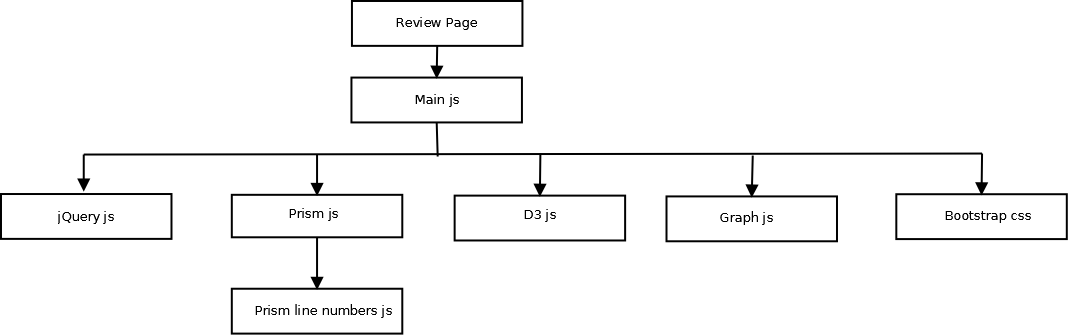
\includegraphics[width=400px]{js_dependencies.png}}
  \caption{Dependencies of the used javascript libraries}
  \label{fig:jsdependencies}
\end{figure}

Fortunately not all views require dynamic user interaction and as a result the
crux of the javascript code base is isolated to just one view, the cheaters\_review.html page, where lecturers review code from student submissions marked for plagiarism and then decide to record students as having cheated or not. The following paragraph details the view and the javascript implementation to achieve the interaction, all remaining views do not need dynamic javascript interaction and perform relatively straight forward CRUD (Create, Read, Update and Delete) operations on the database.

\subsection{Dynamic interaction for reviewing cheaters}

The purpose of the cheaters\_review.html view is to display instances of
possible cheating. An instance is a pair of submissions which are similar to one
another, and as a result the data we work with is a list of pairs of students
each with their notably similar submission. The students in a pair are each
rated by a percentage of common lines of code to the total number of lines in
the submission.

This list of pairs tends to be long, and the lecturer needs to be able to intuit the degree of plagiarism by the ratings which are provided. It was detailed in a client review meeting that the use case for this is by observing the rating of the top few listings and tracing down the list for as long as the level remains more or less consistent. When the level falls off drastically it can be assumed that the likelihood of cheating for the remaining students does so as well. To aid  in determining where this threshold lies a histogram is displayed, to the right of the list of pairs, illustrating the number of students in the different percentage ranges.

\begin{figure}[H]
  \center{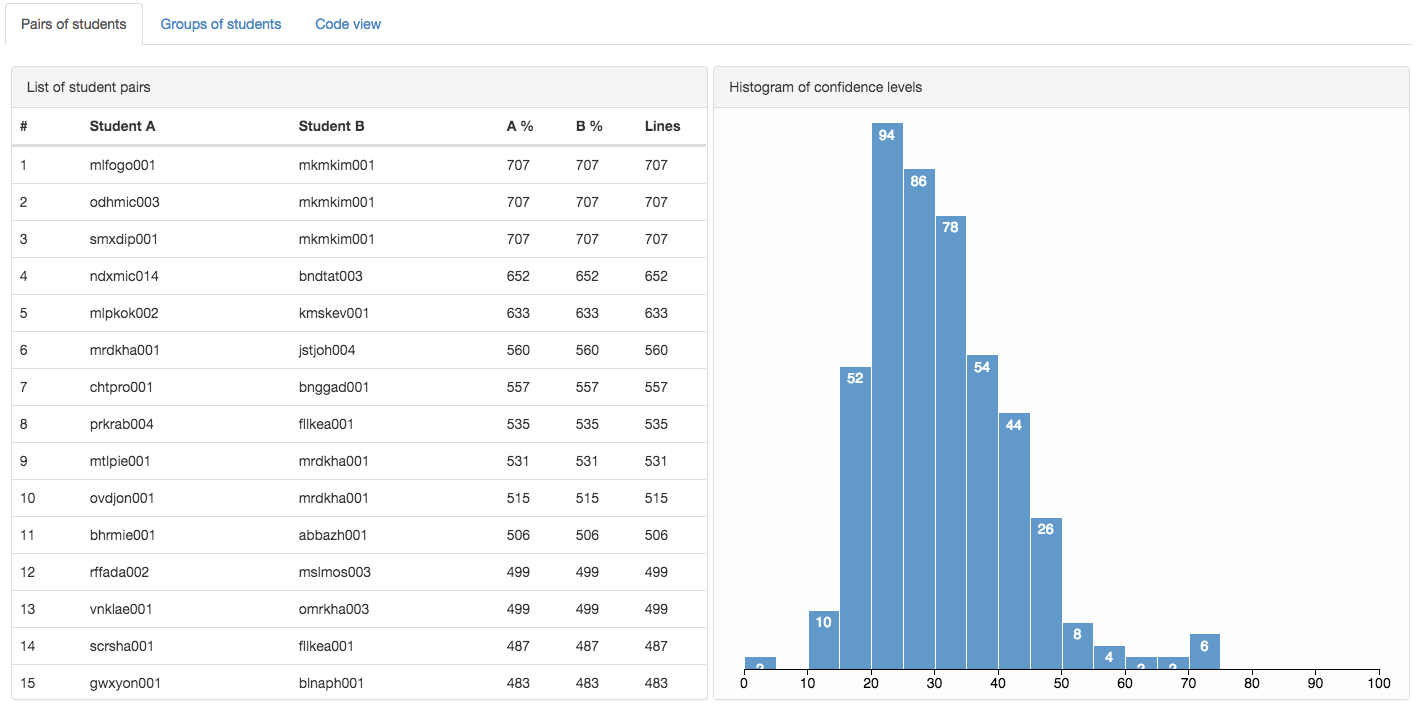
\includegraphics[width=\textwidth]{pairs_histogram.png}}
  \caption{A screenshot of the pairs of students and the corresponding histogram}
  \label{fig:pairshistogram}
\end{figure}

When a lecturer wants to compare code they just have to click on a list pair and the view will switch its focus to a code view displaying the code of the two students side by side. The exact line numbers which match are fetched asynchronously and displayed clearly in highlighted blocks over the code. Above the code blocks there is an action bar which contains dynamically rendered buttons containing the common line numbers, and will scroll the code to the respective line number when clicked.

\begin{figure}[H]
  \center{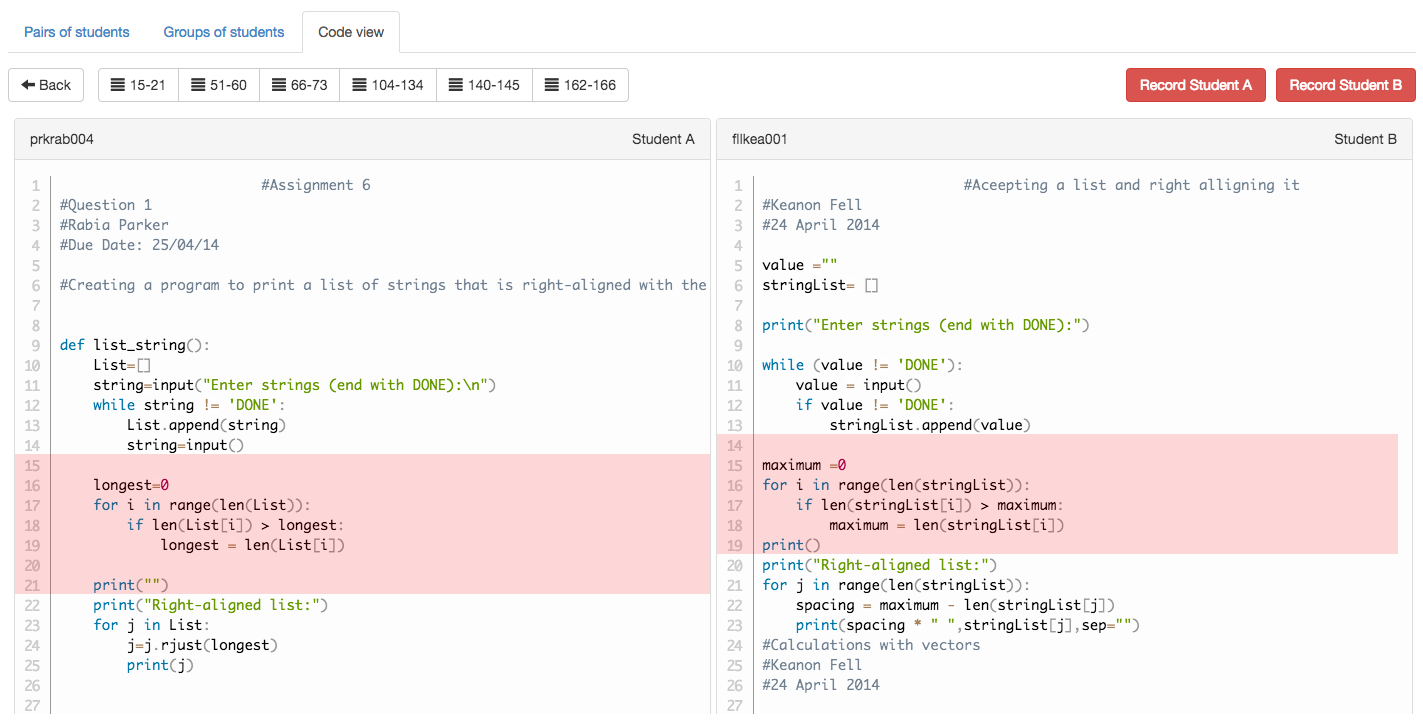
\includegraphics[width=\textwidth]{code_view.png}}
  \caption{A screenshot of the copied regions of code}
  \label{fig:codeview}
\end{figure}

Horizontal and vertical scrolling in the left code block is mirrored by the right code block. This is a design decision made due to the fact that line numbers do not match up one-to-one and are sometimes offset by a fair amount. It is also a result of a limitation with the javascript plugin used for the code highlighting. The design decision is a compromise which allows the user to reach highlighted lines of code in the left block, and then scroll independently in the right code block to make up the offset and view the lines side by side. If scrolling was mirrored in a bidirectional fashion it would be somewhat impractical.

Two buttons exist in the action bar for recording either student independently as having cheated. This is necessary for the use case where the lecturer determines that only one student has cheated. The buttons trigger an asynchronous request to record the respective student as a cheater for the given assignment. The text in the buttons responds accordingly and reflects the state of the request. For example, the button text could read “Record Student A”, upon click that will change to “Recording…” and on successful completion will change to “Undo”. “Undo” means that the transaction has been successful, and it can be reverted if this was made unintentionally by human error. Pressing the button while in the “Undo” state will send an asynchronous delete request and revert the system back to it’s original state. This serves our operability requirement in providing reversible actions and constant feedback.

\begin{figure}[H]
  \center{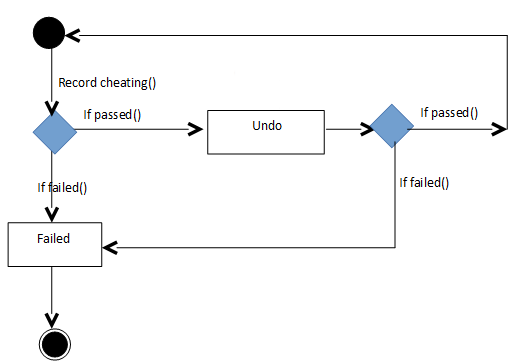
\includegraphics[width=250px]{report_button_state.png}}
  \caption{State diagram of Report buttons}
  \label{fig:statediagram}
\end{figure}


A back button is provided in the action bar to conveniently return back to the previous listing and continue after the lecturer has finished reviewing the code.

\subsection{Listing students in Groups}

It is often the case that code is shared among a group of students, not just
two. The listing of student pairs is linear and provides no information as to
the relationship among student pairs. It is useful for the lecturer, and a
requirement of the system, to be able to see the extent of cheating by knowing
about these groups of students with similar code. To meet this requirement we
have an additional listing containing Groups of student pairs. This listing is
built upon the data containing the student pairs and feeds the pairs into a
graph with the students as nodes and the pair as the edge connecting them. The
graph is then traversed and it identifies groups as isolated clusters of
students. These groups are then listed, containing the pairs that make up the group. Clicking on a pair in a group will render the graph representing the entire group into the diagram on the right of the group listing. This graph gives a visual illustration of how the group is related and a star shaped graph quickly identifies the student most likely to have shared the code. Clicking on an edge in the graph will select the pair and focus the view onto their code in precisely the same way as in the Pairs listing.

\begin{figure}[H]
  \center{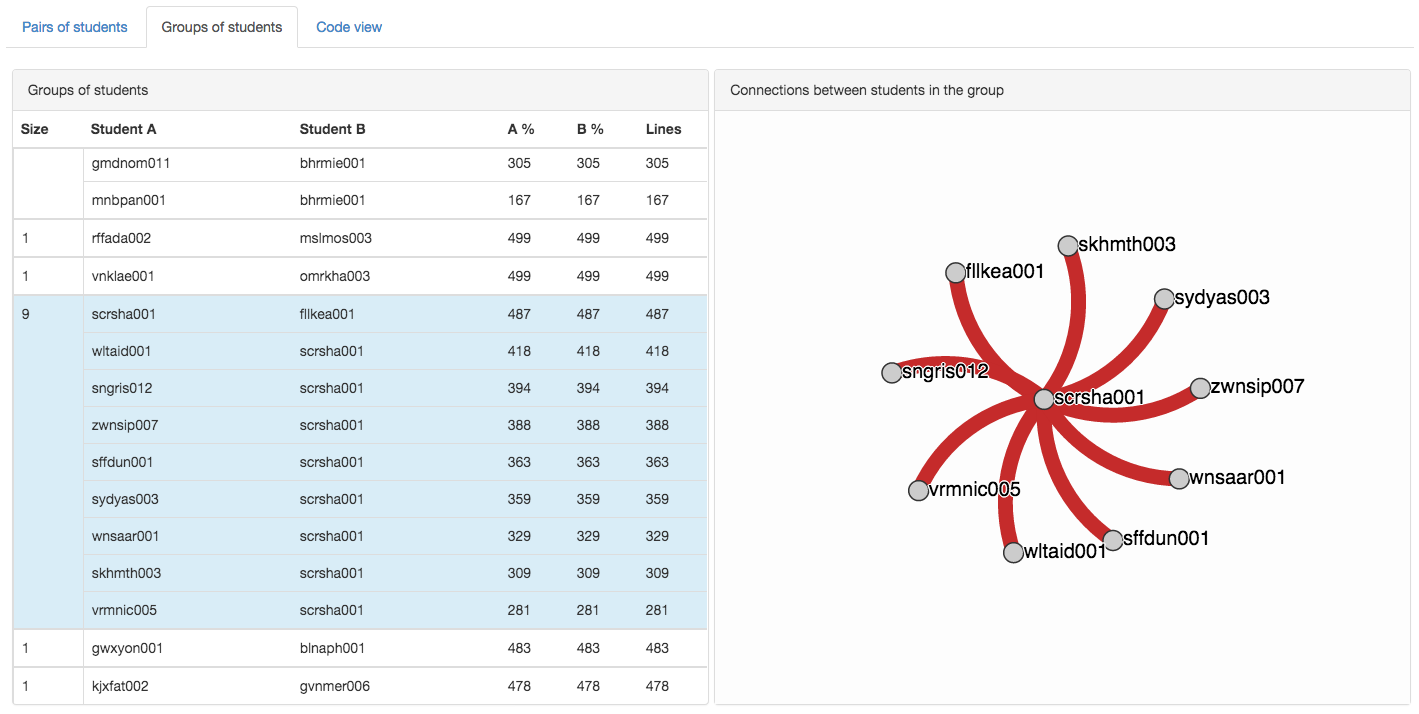
\includegraphics[width=\textwidth]{group_view.png}}
  \caption{A screenshot of the group view with a star topology graph}
  \label{fig:graphview}
\end{figure}

\subsection{Reports on cheating students}

A use case for acting on instances of cheating is to manually copy the offending
student numbers over into an excel spreadsheet. This spreadsheet is then
referenced when assigning students zero or taking further action on them. The
system meets this use case by providing a report page which lists the students
that have been marked for cheating per assignment. A button is provided on the report pages which will download the list as a CSV file in the case where a lecturer needs to use the data elsewhere. The downloaded CSV file is named according to the assignment number for easy identification. A button also exists to delete students from the listing. This is either in the case where a student has been added in error, or the student has been resolved or assigned zero and no longer needs to be listed.

\begin{figure}[H]
  \center{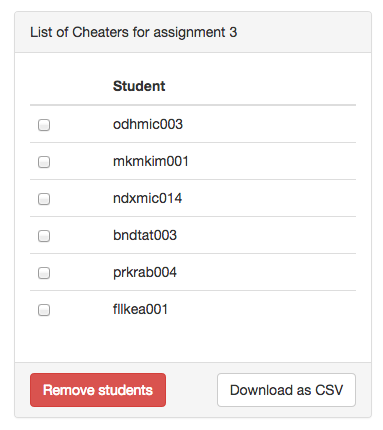
\includegraphics[height=200px]{report_view.png}}
  \caption{A screenshot of the report view, listing students that have been
  marked as cheating on an assignment}
  \label{fig:reportview}
\end{figure}

\begin{figure}[H]
  \center{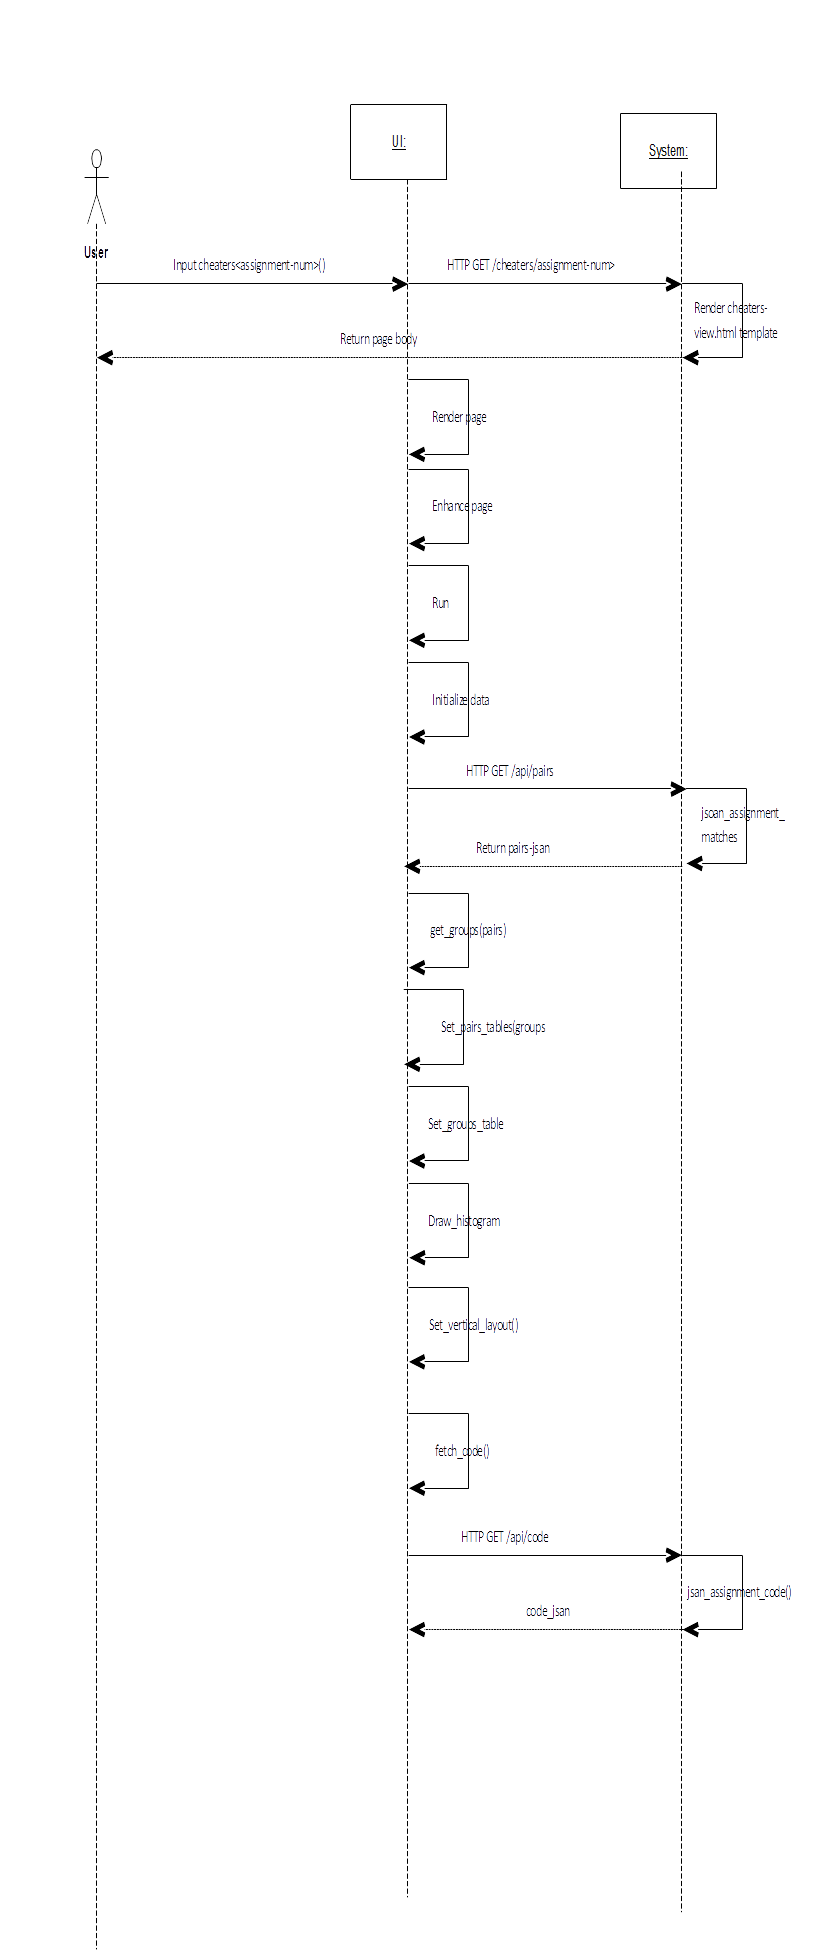
\includegraphics[height=600px]{ui_sequence_diagram.png}}
  \caption{Sequence diagram of main.js of page load}
  \label{fig:uisequence}
\end{figure}


\section{General overview of the entire system}

\begin{figure}[H]
  \center{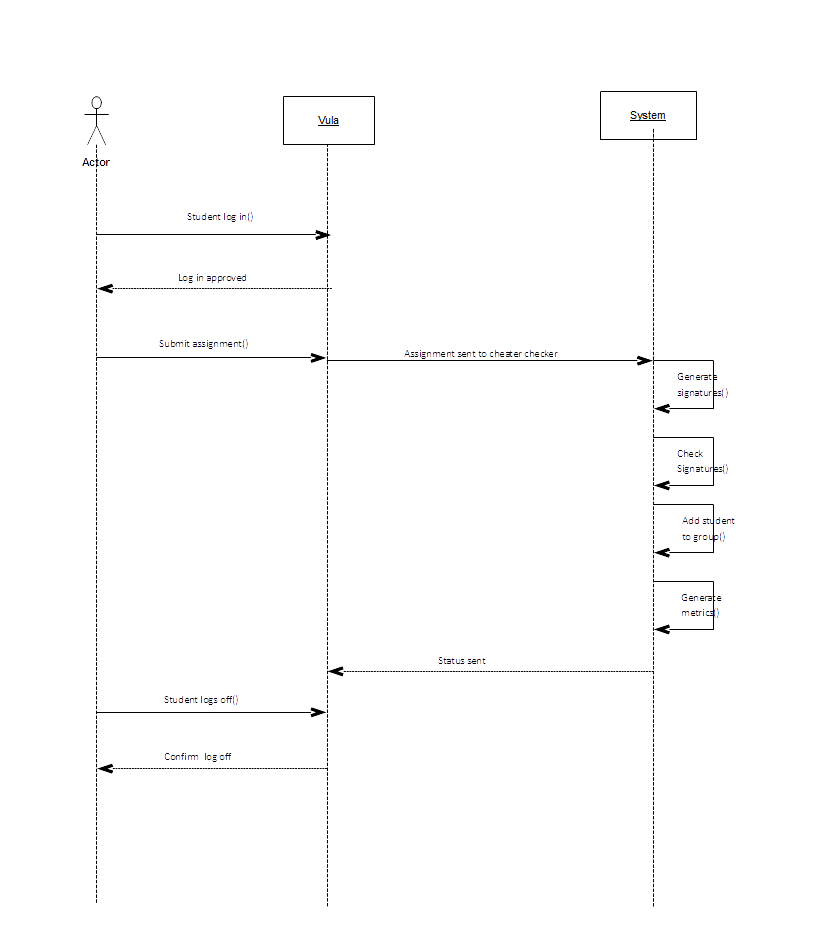
\includegraphics[width=\textwidth]{sequence_diagram.png}}
  \caption{A sequence diagram to indicate how the system works}
  \label{fig:sequencediagram}
\end{figure}

\paragraph{All classes are grouped into groups based on their use. The groups of
classes are}
\begin{itemize}
\item Algorithms
\item Database
\item External
\item Languages
\item Model
\item Scraper
\item Tests 
\item UI
\end{itemize}

\subsection{Relationship between classes}

\textit{BaseAlgorithm abstract class}\\ 
Abstract class for detection algorithm which defines methods.\\

\textit{WinnowingAlgorithm extends BaseAlgorithm}\\
Implements a string matching algorithm (similar to the one implemented by the
JMoss system) for signature generation and signature matching.\\

\textit{Program}\\
Represents a submission by the user and stores our cheating detections\\

\textit{PythonProgram extends Program}\\
Implements Python specific parsing to remove variable and function names\\

\subsection{Special programming techniques}

Test driven development was used to make code more efficient and reduce occurrences of errors in the code. Automated testing was used for this same reason, to catch bugs as they occurred.

\subsection{Libraries}

Libraries plyj and  ply were used to parse code from submissions to the system to be evaluated. Sqlite3 was used for database management. Flask was used as a web framework for the presentation layer of the system and to make calls to the database manager.


\section{Program Validation and Verification}
\label{ss:progr-valid-verif}

We wrote automated unit tests to verify that our code is correct and valid. Unit tests check that for a given input our methods and classes behave as expected. Inputs were method specific and any incorrect data was ignored with the use of try, catch statements. Random incorrect data is hard to come by given that the system simplifies inputs to methods as much as possible. 

\begin{table}[H]
  \centering
\caption{A table of tests. A table caption goes above the table.}

  \begin{tabular}[t]{|p{5cm}|p{3cm}|p{3cm}|p{3cm}|} 
      \hline 
          \textbf{Data Set and reason for its choice} & 
          \multicolumn{3}{c|}{\textbf{Test Cases}}
          \\
          \cline{2-4} & 
            \emph{Normal Functioning} & 
            \emph{Extreme boundary cases} &
            \emph{Invalid Data (program should not crash)} 
          \\ 
          \hline 
            Syntax error in submission file & 
            Passed & 
            Syntax errors & 
            Ignored
          \\
          \hline 
            Database management testing &
            Passed &
            Invalid inputs were ignored &
            Removed to ensure normalisation
          \\ 
          \hline
            Detection algorithm testing &
            Passed &
            &
          \\ 
          \hline
            Flask server testing &
            Passed &
            n/a &
            None
          \\
          \hline
              Testing the suffix tree &
              Passed &
              &
          \\
          \hline
            Testing the suffix tree algorithm &
            Passed &
            Long files were passed to the algorithm. &
            None
          \\
          \hline
            Testing the winnower algorithm &
            Passed &
            None &
            None
          \\
          \hline
            Test the canonicalisation &
            Passed &
            None &
            None
          \\
          \hline
          Test the Runner &
          Passed &
          &
          \\
          \hline
  \end{tabular}

\label{tab:tests}
\end{table}

The system is sensitive because certain sets of inputs can cause the
system to fail. Try, catch statements are used to bypass syntax errors in code
submissions, allowing the system to continue processing remaining submissions.
It is assumed that submissions are parsed through the automatic marker and the automatic marker wouldn't have accepted the syntax error either. The rest of the tests ran on the same principle in that inputs were supplied to ensure basic functionality. In essence basic functionality was all that was required as the system was specific enough to make sure that inputs supplied to the methods would be as simplified as possible. As an example of the simplification, the canonicalisation method takes a .zip folder and reduces it to one exceptionally long string and the string is then manipulated.

\section{Conclusion}
\label{ss:conclusion}

The initial aim of this project was to ensure optimal functionality of the system in terms of algorithm, speed, usability and user experience. Usability and user experience were well met in that the user interface has been designed to incorporate all necessary data in a simple layout which enhanced user experience. User experience success relies on the intuitive design and how easy it is to familiarize oneself with the system which was achieved. The speed and optimization of the algorithm was fairly well met. The expected time taken per submission was a little under what we expected however in practical use, it will be substantially faster in that one submission will be processed at a given time rather than every assignment we were given. The degree of achieving a successful system is fairly high. The system has withstood all tests and works efficiently. The code was structured as indicated using the object orientation standards and general layout. Thus, this project has been a combination of success in learning how to build the system and for a user to implement the system.

\begin{thebibliography}{51}

\bibitem{Burrow} [Burrows, S., Tahaghoghi, S. M., \& Zobel, J. (2007)]
Efficient plagiarism detection for large code repositories. Software: Practice and Experience, 37(2), 151-175.

\bibitem{schleimer} [Schleimer, S., Wilkerson, D. S., \& Aiken, A. (2003, June)]
Winnowing: local algorithms for document fingerprinting. In Proceedings of the 2003 ACM SIGMOD international conference on Management of data (pp. 76-85). ACM.

\bibitem{frohlich} [Frohlich,P.H (2013,3)]
Assignment 4: Semantic Analysis/ Abstract Syntax Tree. 
http://gaming.jhu.edu/~phf/2013/spring/cs328/assignment-ast.shtml

\bibitem{unknown1} [Unknown (2012,3)]
PowerShell Hash Tables 
http://www.bonusbits.com/main

\bibitem{unknown2} [Unknown(2011,11)]
Store/retrieve a data structure
http://stackoverflow.com/questions/8300364/store-retrieve-a-data-structure

\end{thebibliography}

\section{Appendix A: User manual}

The user enters the system on the home page. The home page consists of a list of
assignments with all the submissions and the pairs of students suspected of
cheating as well as the option of creating, editing and deleting an assignment.
The user can select the desired assignment to view all relevant data to be
sorted through and mark students as cheated. The home page has also incorporated
the report aspect. The report aspect shows all students marked for cheating by a
lecturer in a specific assignment. 

To manage assignments from the home screen, the user can click the "Manage
Assignments" button which will redirect them to the corresponding web page where
they have an option of creating an assignment, editing a selected assignment or
deleting an assignment. To create an assignment, the user must enter all
required data and then click submit. To edit, an assignment must be selected and
then the desired fields to be changed can be edited and saved. To delete an
assignment, the user must select an assignment and click the delete button.

To access the student submission data from the home page, click on an assignment
link. The initial screen will show the pairs of students which have a high
percentage of cheating confidence. The list is sorted by cheating confidence
from highest to lowest. A histogram is on the right hand side of the pairs to
indicate the general distribution of the confidence levels. The user can click
on any pair and the copied sections of code will be highlighted on the adjacent
code blocks. Horizontal and vertical scrolling allows for viewing code that is
too long to fit neatly in the code block..

There is a navigation tab to view Groups of students. Once clicked, groups of
students will be displayed with the number of students per group as well as a
visual representation on the right of the screen illustrating how they are
related . The colour of a graph edge is related to the percentage of cheating
across the group. Red indicates high for example. Clicking an edge on the graph
will display the corresponding two students' code blocks and highlight similar
lines as before. 

Two buttons in the action bar of the code view labeled "Record student A/B"
serve to mark a student as having cheated. Once a student is marked as cheated,
the student name will be added to a list of students that have been caught
cheating. The report can be generated or viewed at any time. If the lecturer
wishes to take action, the report can be referenced for students who have cheated.  

\end{document}
